% \documentclass[dvipdfmx,autodetect-engine, 12pt]{jsarticle}

% \usepackage{ulem} % 取消線を引くためのパッケージ
% \usepackage[dvipdfmx]{graphicx} % 画像を挿入するためのパッケージ
% \usepackage{array} % 表の幅指定や自動改行に必要
% \usepackage{enumitem}

% % --- 参考文献用の設定 ---
% \usepackage[backend=biber, style=numeric]{biblatex}
% \addbibresource{../source.bib}
% \usepackage{url}

% % --- section の文字サイズを調整 ---
% \makeatletter
% \renewcommand{\section}{%
%   \@startsection{section}{1}{\z@}%
%     {1.5ex\@plus.5ex\@minus.2ex}%
%     {0.5ex\@plus.3ex}%
%   {\normalfont\normalsize}%
% }
% \makeatother

% \begin{document}

% タイトル
\begin{center}

{\LARGE \bfseries 発展課題 ファイアウォールの構築\par}

\end{center}

\vspace{1cm}

{\LARGE \uline{目的}} \\

\hangindent=1.5zw
\hangafter=0
\noindent
iptables を用いたパケットの制御の実習を行う. パケットを分析することによりファイアウォール設定の正しさを確認する．


\vspace{1cm}

{\LARGE \uline{事前準備}} 

\begin{itemize}
    \item 2 つの VM を起動する．
    \item iptables コマンドについて調査する
\end{itemize}

\vspace{1cm}

{\LARGE \uline{注意事項}} \\

\hangindent=1.5zw
\hangafter=0
\noindent
自分で構築，設定していない IP アドレスのマシンへの通信が勝手に発生している場合は，解析に含めなくてよい

\vspace{1cm}

{\LARGE \uline{操作手順例}} 



\begin{enumerate}
    \item 全ての iptables の設定を消去する．
    \item router で dropbear が起動していないことを確認する．起動している場合には停止させる．
    
        \vspace{\baselineskip}
        \quad
        図\ref{fig:router_no_dropbear}にrouterにおいてdropbear
        という文字列を含むプロセスの一覧を確認するコマンドを実行した結果を示す.

        \begin{figure}[htbp]
            \centering
            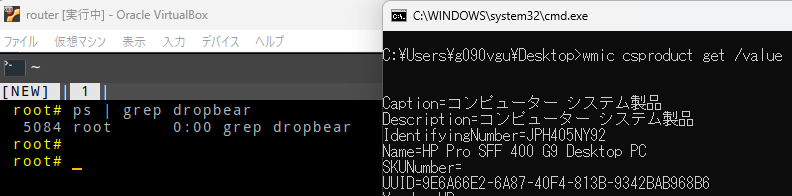
\includegraphics[width=0.8\textwidth]{imgs/no_dropbear_router.png} 
            \caption{routerにおけるdropbearという文字列を含むプロセス一覧}
            \label{fig:router_no_dropbear}
        \end{figure}

        \quad
        実行結果から, プロセス一覧表示に使用したgrepの文字列検索以外の
        プロセスが表示されていないことから, routerにおいてdropbearは起動していないことがわかる.
        \vspace{\baselineskip}

    \item iptables を設定し，router への全てのインターフェースに対する通信に対し，下記のように処理するように設定する．必要であれば sysctl によって転送の許可を行う ．
    \begin{enumerate}
        \item 全ての通信を遮断する
        \item ただし， TCP2000 番ポートへのアクセスには応答できるようにする．
    \end{enumerate}

        \vspace{\baselineskip}
        \quad
        図\ref{fig:iptables_setting}に手順1, 3の操作結果を示す.
        \begin{figure}[htbp]
            \centering
            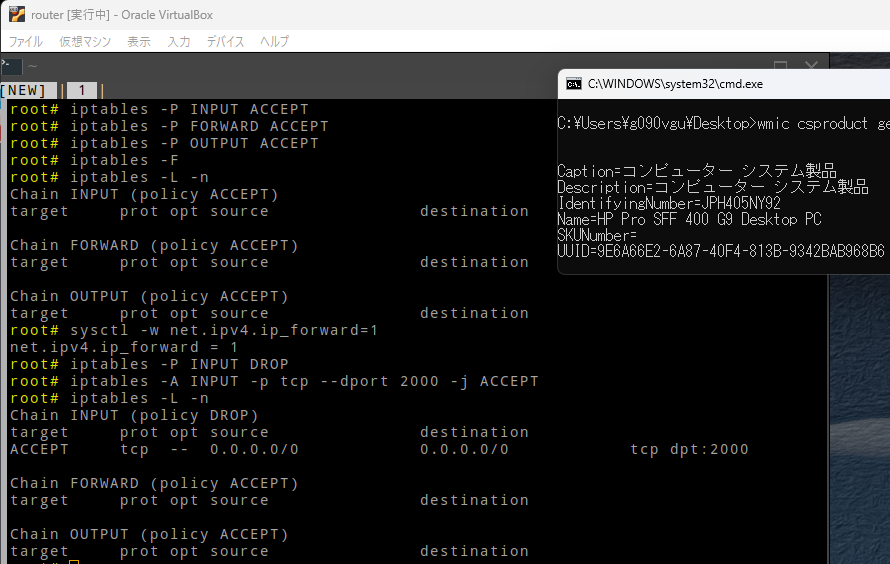
\includegraphics[width=0.8\textwidth]{imgs/init_and_set_iptables.png} 
            \caption{iptablesの設定の消去と設定}
            \label{fig:iptables_setting}
        \end{figure}

        \quad
        まず, -Pオプションによって対象のチェインのポリシーを設定している.
        ここではfilterテーブル上のすべてのチェイン(INPUT, FORWARD, OUTPUT)に対してACCEPTというポリシーを設定し,
        デフォルトですべてのパケットを通過するよう設定している\cite{man:iptables}.\\
        \quad
        次に, -Fオプションを用いてチェイン上のルールをすべて消去している.
        ここでは特にチェインを指定していないため, filterテーブル内のすべてのチェインのルールを全消去し\cite{man:iptables}, 
        -Lオプションを用いてfilterテーブル内のすべてチェインにあるすべてのルールを全表示することによって
        filterテーブル内のすべてのチェインのルールが消去されていることを確認している\cite{man:iptables}.\\
        \quad
        続いて, 要件\textcircled{1}を満たすため, INPUTチェインのポリシーをDROPに設定し, 
        要件\textcircled{2}を満たすため, 
        
        

        \vspace{\baselineskip}


    \item router で TCP 22 番，2000 番ポートを用いて SSH 通信が行えるように dropbear を起動させる．適宜，必要なオプションを用いること．dropbear が 2 つ起動していることを確認すること．
    
        \vspace{\baselineskip}
        図\ref{fig:processes_including_dropbear}にdropbearという文字列を含むプロセスの一覧を示す.
        \begin{figure}[htbp]
            \centering
            
\includegraphics[width=0.8\textwidth]{imgs/dropbear_2_process.png} 
            \caption{dropbearという文字列を含むプロセスの一覧}
            \label{fig:processes_including_dropbear}
        \end{figure}
        \vspace{\baselineskip}

    \item router で Wireshark を起動し，組織内のインターフェースの通信を解析できるようにキャプチャする interface を設定する．
    \item server から router の 22 番，2000 番ポートに SSH でアクセスする過程のパケットを，router で起動した Wireshark で解析し，通信が許可されたポートでのみ通信が可能で，許可されていないポートでは通信ができないことを，実験した結果を用いて，レポートで報告しなさい．
    
        \vspace{\baselineskip}
        図\ref{fig:processes_including_dropbear}にdropbearという文字列を含むプロセスの一覧を示す.
        \begin{figure}[htbp]
            \centering
            
\includegraphics[width=0.8\textwidth]{imgs/ssh_22.png} 
            \caption{ポート22にsshログインを試みた結果}
            \label{fig:ssh_22}
        \end{figure}
        \begin{figure}[htbp]
            \centering
            
\includegraphics[width=0.8\textwidth]{imgs/ssh_2000.png} 
            \caption{ポート2000にsshログインを試みた結果}
            \label{fig:ssh_2000}
        \end{figure}
        \vspace{\baselineskip}
\end{enumerate}

\newpage

% % 参考文献
% \printbibliography[title=参考文献]

% \end{document}
